%%%----------- Preamble ----------
\documentclass[times, 1pt, a4paper]{article}

\usepackage[top=1.5in, bottom=1.5in, left=1.2in,right=1in]{geometry} % Margin
\usepackage{graphicx} % Figures
\usepackage{epstopdf}
\usepackage{verbatim}
\usepackage{enumitem}
\usepackage{multirow} % Multirow
\usepackage{tabularx}
\usepackage{epsfig}
%\usepackage{tipa}
\usepackage{slashbox,multirow} 
\usepackage{float}
\usepackage{lscape}
\usepackage{caption}
\usepackage{amssymb,amsmath}
\usepackage{setspace}
\usepackage{rotating}
\usepackage{mathpazo}


%%% For hyper reference
\usepackage{hyperref}
\hypersetup{
    colorlinks,
    citecolor=black,
    filecolor=black,
    linkcolor=black,
    urlcolor=black
}

\setcounter{secnumdepth}{3}
\setlist{nolistsep}
\linespread{1.25}
\textheight 8.8in
\textwidth 6.2in

%------ Document body ---------



\begin{document}

\title{\fontsize{16pt}{19.2pt}\selectfont\bf{Development of an Integrated Framework for Investigating Healthcare Data Using Natural Language Processing and Big Data Analytics}}
\date{}

\maketitle
\thispagestyle{empty}

\begin{center}
\vspace*{-8mm}
\textit{Project report submitted in partial fulfilment of the requirements for the partial completion of}

\vspace*{6mm}

{\fontsize{14pt}{16.8pt}\selectfont\textbf{PROJECT WORK - II [11EC8DCPRJ]}} \\ \vspace*{3mm}
{\fontsize{14pt}{16.8pt}\selectfont\textit{in}} \\
\vspace*{3mm}
%
{\fontsize{14pt}{16.8pt}\selectfont\textbf{ELECTRONICS AND COMMUNICATION ENGINEERING}} \\

\vspace*{2mm}
{\fontsize{14pt}{16.8pt}\selectfont\textit{by}} \\
\vspace*{3mm}

\author{\fontsize{14pt}{16.8pt}\selectfont\textbf{Achutananda M P}}  \hspace*{12mm} {\fontsize{14pt}{16.8pt}\selectfont\textbf{Harikrishna D M}}\\
\vspace*{2mm}
{\fontsize{12pt}{14.4pt}\selectfont\textit{[Roll No. 1BM18EC300]} \hspace*{12mm} \selectfont\textit{[Roll No. 1BM18EC301]} } \\



\vspace*{3mm}

\vspace*{4mm}\fontsize{14pt}{16.8pt}\selectfont\textit{Under the supervision of} \\
\vspace*{2mm}\fontsize{14pt}{16.8pt}\selectfont\textbf{Latha H N} \\
\vspace*{8mm}

\begin{figure}[!ht]
\centering

\includegraphics[height=36.068mm,width=33.274mm]{VTU_Logo}
\end{figure}

\vspace*{3mm}

\fontsize{14pt}{16.8pt}\selectfont\textbf{Department of Master of Computer Applications  \\
\vspace*{2mm} R.V.  COLLEGE OF ENGINEERING, Mysore Road} \\
\vspace*{2mm}
\fontsize{14pt}{16.8pt}\selectfont\textbf{Bengluru-560059, India} 
\vspace*{10mm}\\

\end{center}
 %cover page
\thispagestyle{empty}
\newpage

{\fontsize{16pt}{19.2pt}\selectfont\bf{\begin{center}
DECLARATION
\end{center}}}

\vspace*{1cm}

We undersigned students of final semester B.E in Electronics and Communication Engineering and Electrical and Electronics Engineering, BMS College of Engineering, Bangalore, hereby declare that the dissertation entitled \textit{``IMPLEMENTATION OF A SMART TROLLEY"}, embodies the report of the project work carried out independently by us under the guidance of Mrs. Latha H N, Assistant Professor,  E\&C Department, BMSCE, Bangalore in partial fulfilment for the award of Bachelor of Engineering in Electronics and Communication from Visvesvaraya Technological University, Belgaum during the academic year 2017-2018.

We also declare that to the best of our knowledge and belief, this project has not been submitted for the award of any other degree on earlier occasion by any student.

\vspace*{1cm}

\begin{flushleft}
Place: Bangalore \\
Date: \date{\today{}}
\end{flushleft}

\vspace*{1cm}

\begin{flushright}
{\fontsize{14pt}{16.8pt}\selectfont\textbf{Achutananda M P}}  \hspace*{12mm} {\fontsize{14pt}{16.8pt}\selectfont\textbf{1BMEC300}}\\
\vspace*{3mm}
{\fontsize{14pt}{16.8pt}\selectfont\textbf{Harikrishna D M}}  \hspace*{12mm} {\fontsize{14pt}{16.8pt}\selectfont\textbf{1BMEC301}}\\
\end{flushright}


 %cover page
\thispagestyle{empty}
\newpage


\vspace*{1.5cm}

\begin{center}

\vspace*{2mm} \fontsize{14pt}{16.8pt}\selectfont\textbf{B.M.S COLLEGE OF ENGINEERING} \\
\vspace*{2mm}
\fontsize{14pt}{16.8pt}\selectfont\textbf{Department of Electronics and Communication Engineering} 
\vspace*{10mm}\\

\begin{figure}[!ht]
\centering

\includegraphics[height=36.068mm,width=33.274mm]{figures/BMS_Logo.png}
\end{figure}

\end{center}

\noindent This is to certify that the project entitled \textit{``IMPLEMENTATION OF A SMART TROLLEY"} is a bonafide work carried out by \textbf{Achuthananda M P} (USN:1BM18EC300) and \textbf{Harikrishna D M} (USN:1BM18EC301) in partial fulfillment for the partial completion of \textit{PROJECT WORK - II [11EC7DCPW1]} during the academic year 2017-2018.
 

\vspace*{2.5cm} 

\begin{tabular}{p{5cm}p{5cm}p{5cm}}
\textbf{Latha H N} & \textbf{Dr. G. Poornima} & \textbf{Dr. K.Mallikharjuna Babu} \\
{\fontsize{12pt}{14pt}\selectfont\textit{Asst. Prof.}} &  {\fontsize{12pt}{14pt}\selectfont\textit{HOD}} & {\fontsize{12pt}{14pt}\selectfont\textit{Principal}} 

\end{tabular}
 
\vspace*{2.5cm}

External Examiner \hfill Signature with date

\thispagestyle{empty}
\newpage

{\fontsize{16pt}{19.2pt}\selectfont\bf{\begin{center}
ACKNOWLEDGEMENT
\end{center}}}

\vspace*{1cm}

Any achievement, be it scholastic or otherwise does not depend solely on the individual efforts but on the guidance, encouragement and cooperation of intellectuals, elders, and friends. Several personalities, in their own capacities have helped us in carrying out this project work. We would like to take this opportunity to thank them all.

We express profound gratitude to respected principal Dr. K. Mallikharjuna Babu, BMS College of Engineering for providing a congenial environment to work in. Our sincere gratitude to Dr. G Poornima, Head of the Department, Electronics and Communication Engineering for encouraging and providing this opportunity to carry out the project in the department.
We would like to thank our guide Ms. D.R. Ambika, Assistant Professor, Department of ECE who helped us in all the ways to carry out the project work. She stood beside and guided us in every step. 

We thank all our professors for providing the basic knowledge without which this project wouldn't have been possible. Last but not the least we thank our family and friends, who made their valuable support compelled us to maintain a standard throughout our endeavour.

\vspace*{1cm}

\begin{flushleft}
Achutananda M P \\
Harikrishna D M 
\end{flushleft}

\thispagestyle{empty}
\newpage

{\fontsize{16pt}{19.2pt}\selectfont\bf{\begin{center}
ABSTRACT
\end{center}}}

\vspace*{1cm}

In today’s world, there is a constant quest to minimize the work of humans, save labor, conserve energy, and improve the accuracy, quality, and precision of any work. This leads to automation. Automation or automatic control is the use of various control systems for operating equipment or for completing a task with minimal or reduced human intervention. Some processes are completely automated while others are partially automated, depending on the task. Several industries have already automated their manufacturing units and assembly units, drastically reducing costs and increasing their outputs. An industry that can benefit from such automation is the Retail/ Supermarket industry.


Lots of people use supermarkets. These supermarkets can get crowded during festivals, special occasions or even during rush hours every day. While it is great for the supermarket to have so many people willing to buy at their store, increasing its revenue, the long lines at billing counters can be a great deterrent for potential customers. Long lines have a tendency to drastically reduce perceived customer satisfaction. It could even mean some potential customers may decide to give up and leave the store without buying anything. In fact, lines that are "too long" are the second most common complaint of consumers against retailers (the first complaint being that the members of the staff are "rude"). Surveys have revealed that the customers don’t like waiting in queues because they feel that they are wasting their time and being unproductive. When they finally get their turn at the billing counter, they often meet a rude and harassed employee. This further serves to take away from the overall good impression of the store the customer might have otherwise formed.


While the above problem can be dealt with temporarily by distracting the consumers with strategically placed merchandise or explaining the reason for the delays caused, the root of the problem – long lines doesn’t go away. A feasible solution that might permanently address the problem of long lines is the automation of the billing process.
\thispagestyle{empty}
\newpage

\newpage
\tableofcontents
\thispagestyle{empty}

\newpage
\listoffigures
\thispagestyle{empty}

\newpage
\listoftables
\thispagestyle{empty}

\newpage

\setcounter{page}{1} 

\graphicspath{{figures/}} %path to figures folder

\section{Introduction}\label{section:intro}

Ask any person who goes to the supermarket regularly if they have faced problems with the billing counter. The answer would be a quick `YES!' Long lines tend to drastically reduce perceived customer satisfaction. It could even mean some potential customers may decide to give up and leave the store without buying anything. In fact, lines that are ``too long" are the second most common complaint of consumers against retailers (the first complaint being that the members of the staff are ``rude"). These supermarkets can get crowded during festivals, special occasions or even during rush hours every day. While it is great for the supermarket to have so many people willing to buy at their store, increasing its revenue, the long lines at billing counters can be a great deterrent for potential customers. Surveys have revealed that the customers don't like waiting in queues because they feel that they are wasting their time and being unproductive. When they finally get their turn at the billing counter, they often meet a rude and harassed employee. This further serves to take away from the overall good impression of the store the customer might have otherwise formed.

While the above problem can be dealt with temporarily by distracting the consumers with strategically placed merchandise or explaining the reason for the delays caused, the root of the problem  long lines doesn’t go away. A feasible solution that might permanently address the problem of long lines is the automation of the billing process.

The `Smart Trolley' aims to improve customer shopping experience by cutting down the boring task of standing in queues while providing an interactive experience with the customer. The customer should merely pick up the item and drop it in the trolley, the trolley automatically adds the item to the bill or removes the item from the bill when he removes the item. Once the customer is done shopping, a complete bill of items is presented to the customer right before him on a display. 


This is a reference for figure \ref{fig:barcode}

\subsection*{Barcodes as a Mean of Unique Identification} \label{subsection:barcode}

The challenges that we stumble upon for identification of real world objects for everyday applications are the variations in font, languages, text size, etc. which inspired people to adopt a universal standard called the barcode.

A barcode essentially is a way to encode information in a visual pattern that a machine can read. The combination of black and white bars represents different text characters which follows a set algorithm for that barcode type. If you change the sequence of elements you get different text. A barcode scanner reads this pattern of black and white that is then turned into a line of text your computer can understand. GTIN-13 barcode is shown in Figure \ref{fig:barcode}. 

\begin{figure}[h] 
	\centering
	\resizebox{6cm}{6cm}{
\includegraphics{BMS_Logo}}  
	\centering
	\caption{College Logo}
	\label{fig:coll_logo}
	\end{figure}


  \begin{figure}[h] 
	\centering
	\resizebox{12cm}{6cm}{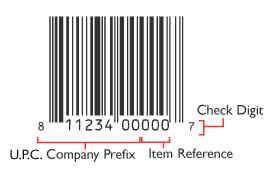
\includegraphics{Fig_Barcode}}  
	\centering
	\caption{GTIN-13 Barcode}
	\label{fig:barcode}
	\end{figure}


Barcodes can be used at applications where visual identification is required like the products at a grocery store, clothing store, college attendance systems, etc. There is a myriad of applications
The GTINs is an identifier of trade items developed by GS1. These identifiers are usually placed on the trade item in the form of a barcode. Such identifiers are used to look up product information in a database which may belong to a retailer, manufacturer, collector, researcher, or other entity. 
The camera in the smart trolley uses the GTIN barcode as a means of identifying the item. The camera must get a glimpse of the barcode while it is being placed inside the trolley by the customer. 


\subsection*{Image Processing} \label{subsection:image_processing}

Image processing is a method to convert an image into digital form and perform some operations on it to extract some useful information from it. It is a type of signal dispensation in which input is image, like video frame or photograph and output may be image or characteristics associated with that image. Usually Image Processing system includes treating images as two dimensional signals while applying already set signal processing methods to them. 
It is among rapidly growing technologies today, with its applications in various aspects of a business. Image Processing forms core research area within engineering and computer science disciplines too.

Image processing basically includes the following three steps.

\begin{itemize}
\item Importing the image with optical scanner or by digital photography.
\item Analyzing and manipulating the image which includes data compression and image enhancement and spotting patterns that are not to human eyes like satellite photographs.
\item Output is the last stage in which result can be altered image or report that is based on image analysis.
\end{itemize}


The purpose of image processing is divided into 5 groups. They are:

\begin{enumerate}
\item Visualization - Observe the objects that are not visible.
\item Image sharpening and restoration - To create a better image.
\item Image retrieval - Seek for the image of interest.
\item Measurement of pattern – Measures various objects in an image.
\item Image Recognition – Distinguish the objects in an image.

\end{enumerate}
     

\subsection*{Problem Definition} \label{subsection:problem_definition}

To develop a system which performs the task of automation of scanning of barcodes present on objects and the billing process that follows. A suitable method must be used for scanning of the barcodes. The item must be detected clearly by the camera. For this purpose, the image of the barcode must be suitably enhanced so that the processor can make sense out of the barcode. The system must detect if the item is inserted or removed by the customer and the entire number of items in the trolley must be verified against a load sensor. The cameras must detect the barcode while it is in motion, hence the quality of the image must be enhanced as the barcode image can get deteriorated due to motion blur. Image must also be neutral to various lighting conditions. Barcodes must be validated before computing the bill.

\subsection*{Proposed Solution} \label{subsection:proposed_solution}

The algorithm developed must detect and decode a barcode on a moving object, obtained from a camera.

\begin{itemize}
\item The camera must be chosen in such a way that it has a frame rate high enough to do justice to capture the object in motion. The camera will be programmed to acquire images at intervals of time such that the frequency is high enough so as to not miss the moving object or produce a blurred image which cannot be manipulated.
\item A suitable way of representing an image, i.e. feature calculations.
\item Image enhancement techniques necessary for the barcode recognition.
\end{itemize}

Validity of the barcode must be checked. i.e. the detected barcode must contain valid information according to universal standards.

The cameras must be triggered at the right time and this method must be reliable. Hence ultra-sonic sensor is used. There are two cameras being used and hence two ultrasonic sensors serve the purpose of triggering the cameras.

For the validation of products being placed or removed from the trolley, a load sensor is used. The sensor is chosen such that it is reliable and is accurate enough for the application. Finally, all the components must be integrated and various test cases for the application must be tested.


Literature review is in Section \ref{section:literature_survey}. Results are in Section \ref{section:results}

\section{Literature Survey} \label{section:literature_survey}

\subsection{Barcode Recognition} \label{subsection:barcode_recognition}

Steffan et al. \cite{zhang2012research} have worked on recognition of 1-D barcodes using cameras of phones. As input, they expect an image containing a ID bar- code which covers the image centre. The barcode does not need to be centered, may be upside down, or may have the usual perspective distortions and rotations (approx. $\pm 15$  degrees) that occur when images are taken by camera phones. 

They assumed a horizontal scan-line in the middle of the image will cover the barcode. If this is not the case, or parts of the barcode which lay on the scan-line are dirty, occluded or affected by strong reflections, they detect this in a very early stage and will repeat the algorithm for alternate scan-lines above and below. 

Without searching for the barcode boundaries, they binarized all pixels on the scan-line in a fast manner, starting from a seed point in the middle. For the binarization a dynamic threshold is required, to be robust against dirt, badly printed barcodes or illumination changes. So, they computed illuminance factor and other dependent parameters to finally compute a threshold for binarization.

They have classified the bars and spaces in the barcodes as digits by first detecting the guard bands followed by checking the sequence of bars and spaces of the left code and right code. For the detection, they took over 1,000 images of barcodes using a camera phone and stored them in a database. Using this fixed set of images, which includes heavily distorted, shaky and out-of-focus pictures, they developed their algorithm which looks for the most similar code from database using MATLAB. 

Their algorithm depends on various factors like illumination which we have eliminated using a feature value. For the detection, they have used a database to check for the most similar code from the database. We have eliminated this by validating the barcode by computing checksum.

\subsection{Feature Calculation} \label{subsection:feature_calculation}

In pattern recognition, each pattern is represented by a set of features or measurements, and viewed as a point in space. Feature vector is an n-dimensional vector of numerical features that represent some object, in this case an image.  Authors Pablo, Claudio and Jacek [3] have worked on the best way to represent an image using feature. 

In their paper titled “Normalized Mutual Information Feature Selection” (Published in IEEE transactions on neural networks, VOL. 20, NO. 2, on February 2009) [3], They have focused on feature selection methods based on Mutual Information (MI) as a measure of relevance and redundancy among features. They aimed at choosing features that allows to discriminate between patterns belonging to different classes. In practice, the optimal set of features is usually unknown, and it is common to have irrelevant or redundant features at the beginning of the pattern recognition process. In general, it is desirable to keep the number of features as small as possible to reduce the computational cost of training a classified as well as its complexity. 

A comparative study was made on various methods of obtaining feature vector. The comparison was made on four data sets: uniform hypercube synthetic data set, Breiman’s waveform data set, spam base data set, and sonar data set. The average normalized mutual information is proposed as a measure of redundancy among features. Normalized Mutual Information Feature Selection (NMIFS) outperformed other methods on several artificial and benchmark data sets without requiring a user-defined parameter. In addition, NMIFS is combined with a genetic algorithm to form a hybrid filter/wrapper method called Genetic Algorithm guided by Mutual Information for Feature Selection (GAMIFS). It is a hybrid filter/wrapper method that combines a genetic algorithm with NMIFS. GAMIFS is able to find both individual relevant features and groups of features that are relevant.

This paper has proposed a method of optimal way of finding the best feature vector based on selecting the most relevant information. In our project, we have implemented a specific method to determine feature vector that eliminates all the computation involved in feature selection.

\subsection{Deblurring Techniques} \label{subsection:deblurring_techniques}

During acquisition, digital images are invariably degraded by a number of phenomena that limit image resolution and utility. Factors that can limit the effective resolution of an imaging system may include aliasing due to under-sampling, blur, and noise. Hence an important aspect of this project involves deblurring of images. Ian Young and Lucas Vliet [2] from Delft University of Technology, Delft, Netherlands have published a paper that talks about an effective implementation of Gaussian filter for deblurring of images. 

In their paper titled “Recursive implementation of the Gaussian filter” (Published in Delft University of Technology, NL-2628 CJ Delft, Netherlands on 29 September 1994) [2], they have proposed a recursive implementation of Gaussian filter. They developed a straightforward recursive implementation of the Gaussian filter. They examined various alternatives and showed that simple forward and backward difference approximations in concatenation lead to the required IIR filter. They also found that their implementation is the fastest of those evaluated and that the result in 2-D (and higher dimensions as well) is isotropic. They developed a simple, algebraic closed-form procedure for choosing the coefficients of the recursive filter which hence determines the behavior of the filter.

Another paper, titled “Restoration of Out of Focus Barcode Images using Wiener Filter” (Published by authors D. Addiati, U. U. Sheikh and S. A. R. Abu Bakar from Universiti Teknologi Malaysia 81310 Skudai, Malaysia on 11 November 2010) [3], describes Wiener filter, which is a proposed solution for deblurring of images. In their paper, they implemented a technique to restore barcode images before the decoding process. This technique involves identification and calculation of Point Spread Function (PSF) parameter and radius of the blur in Cepstrum domain, which is followed by restoration of the degraded image using Wiener filter. Their main objective was to restore barcode images that were affected by out of focus blur. The results were evident about the fact that the method they used was robust and could be applied to any barcode size, direction or the type of barcode. These papers clearly gave us an idea about the various image deblurring techniques which helped us in carrying on with this project.


\subsection{Load Sensor} \label{subsection:load_sensor}

A load cell or a load sensor is a transducer that is used to create an electrical signal whose magnitude is directly proportional to the force being measured. In the paper titled "Load Sensor" [4] (Published by Jorma J Lehtovaara on April 17 2001) the author has spoken about a load sensor which is well suited for measuring belt tension in both idler and torque transmitting pulley assemblies. 

The load sensor, a capacitor type displacement or load sensor includes a first electrode constituted by an electrically conductive coiled spring capable of expansion and contraction and a second electrode positioned to face the first electrode without making contact therewith. The second electrode is constituted by an electrically conductive coiled spring or a cylindrical electric conductor. The sensor is constructed such that capacitance between the first and second electrodes varies with a change of a gap between the first and second electrodes or an opposing area of the first and second electrodes caused by the relative displacement occurring there between.
It is an object of the present invention to provide a sensor in which at least one of two electrodes is in the form of a coiled spring, so that any displacement or load applied externally to the coiled spring can be detected as a capacitance change, thereby making the sensor small and compact and making it possible to attain accurate detection of the displacement or load.

\subsection{Object Detection} \label{subsection:object_detection}

Using cameras for the recognition of barcodes demand the cameras to run continuously while scanning. In case of any other method for scanning of barcodes, the user has control over the duration for which the scanner has to be switched ON. In order to make the system automated, we need to make the cameras run only when required, i.e. when there is an object present in front of it. One way to do this is to use a sensor that can detect the presence of an object in front of it. Anca Discant, Alexandrina Rogozan, Corneliu Rusul and Abdelaziz Bensrhair have spoken about various tecniques used for obstacle detection.

In their paper titled, “Sensors for Obstacle Detection A Survey” (Published in Basis of Electronics Department, Technical University of Cluj-Napoca, Cluj, Romania on 21 January 2008), they tried to identify the main character of an obstacle detection system from the ruttier scene. They classified the main types of sensors from this field in passive (visible and infrared spectrum camera) and active (radar, laser-scanner, sonar) sensors and we made a survey in this domain. A solution for an obstacle detection system was then presented. Almost all obstacle detection systems use a combination of passive-active technology, and in general the best solution is obtained using a vision system combined with a distance sensor like radar or laser. The most low-priced system is one combining only vision systems, but the inconvenient in this case is the lack of distance information. Hence we needed a sensor that is accurate regarding the distance at which the object is placed. Thus an ultrasonic sensor is used for our project.


\section{Methodology and Implementation} \label{section:methodology}

\subsection{Block Diagram} \label{subsection:block_diagram}
 
The basic block diagram is shown in Figure \ref{fig:block_diagram}. 

  \begin{figure}[h] 
	\centering
	\resizebox{14cm}{6cm}{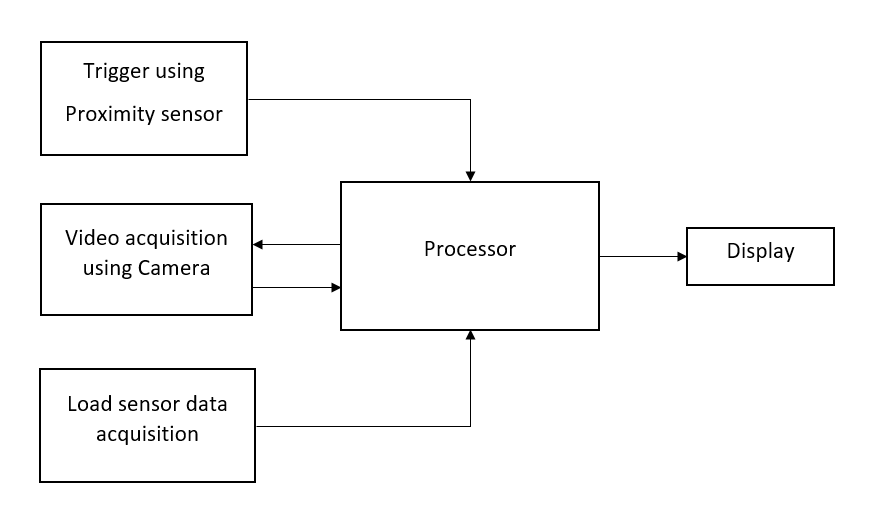
\includegraphics{Fig_Block_Diagram}}  
	\centering
	\caption{Basic block diagram}
	\label{fig:block_diagram}
	\end{figure}




\subsection{Hardware Architecture} \label{subsection:hardware_architecture}

 \begin{figure}[h] 
	\centering
	\resizebox{14cm}{10cm}{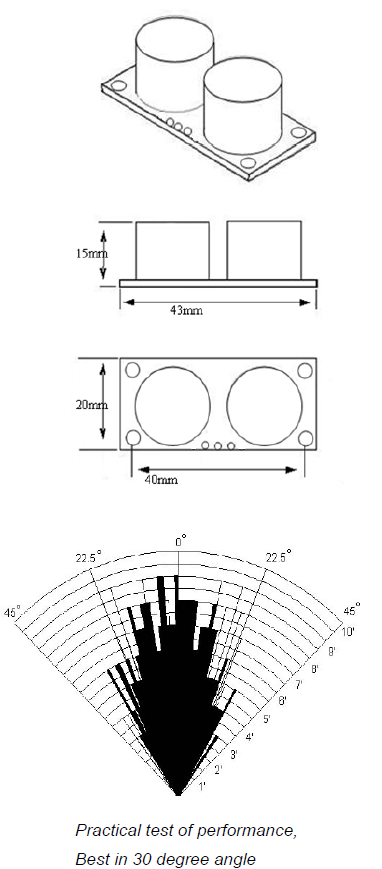
\includegraphics{Fig_HR_S04}}  
	\centering
	\caption{HR-S04}
	\label{fig:hr_s04}
	\end{figure}

The reason for implementation of a trigger is to turn ON the camera only when required, we save power. It is also unnecessary to keep the camera turned ON all the time because the customer enters a product only when he needs to. The proximity sensor can be used in two ways with the cameras. One method is to trigger the camera by the distance from the proximity sensor and the other is to determine the camera by the proximity sensor closest to it. The latter technique is used here. The proximity sensor used here is an ultra-sound sensor which returns the distance from the nearest obstruction. The proximity sensor is programmed using Arduino IDLE. The proximity sensor is programmed in such a way that it returns ‘Triggered’ when the distance between proximity sensor and the object is less than 30cm. 



\begin{table}[h]
\caption {HC-SR04 datasheet \label{table:hr_sr04_datasheet}} 
\centering
\begin{tabular}{|c|c|}
\hline
Supply Voltage & $5\ v$ \\ \hline
Global current consumption & $ 15\ mA $ \\ \hline
Ultrasonic Frequency & $ 40\ KHz $ \\ \hline
Maximal Range & $400\ cm$ \\ \hline
Minimal Range & $3\ cm$ \\ \hline
Resolution & $1\ cm$ \\ \hline
Trigger Pulse Width & $10\ \mu s $  \\ \hline
Outline dimensions & $ 43 \times 20 \times 15 $ \\ \hline
\end{tabular}
\end{table}	

Features of HC-SR04: 

\begin{itemize}

\item Detecting range: 3cm-4m 
\item Best in 30-degree angle
\item Electronic brick compatible interface
\item 5V DC power supply
\item Breadboard friendly
\item Dual transducer
\item Arduino library ready


\end{itemize}

\subsection{Software Architecture} \label{subsection:software_architecture}

 \begin{figure}[h] 
	\centering
	\resizebox{14cm}{10cm}{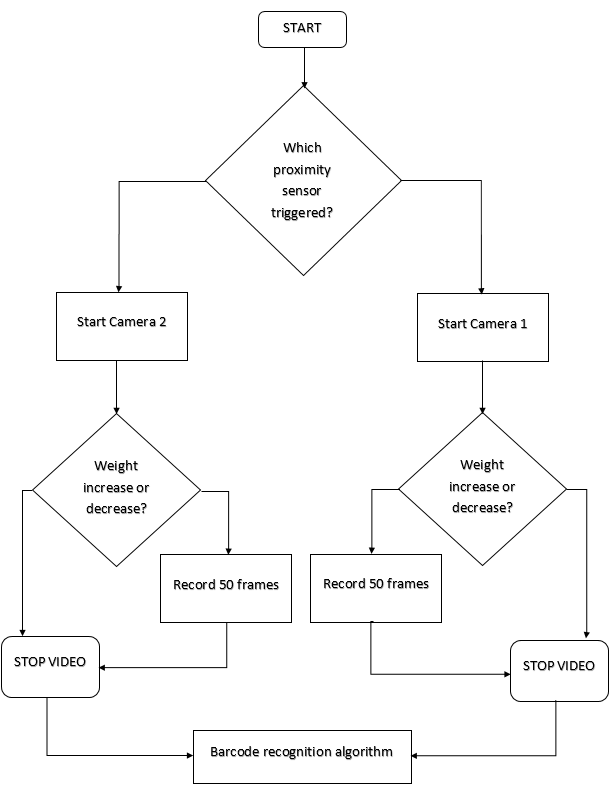
\includegraphics{Fig_SW_Implementation}}  
	\centering
	\caption{Software implementation flowchart}
	\label{fig:software_implementation}
	\end{figure}


The two proximity sensors denote either ‘Triggered’ state or ‘NOT Triggered state’. If the object is within 30cm of the either of the proximity sensor, that proximity sensor outputs a ‘1’. The load sensor denotes ‘Weight increased’ if an item is placed on it and ‘Weight decreased’ if an item is removed from it and ‘No change’ otherwise. Depending on which proximity sensor is triggered, the camera closest to it will start to record a video. The video stops to record when the load sensor outputs ‘Weight increased’. If ‘No change’ the camera records for a certain time before turning OFF. If ‘Weight decreased’ the camera starts to record a new video. This video is then fed to the barcode recognition algorithm.

\subsubsection*{Validation} \label{subsubsection:validation}

Validation is the final process involved in barcode recognition. This is also the most important part. To check whether the given information is valid a code or not, we need to know how information is encoded into a barcode. This project is done for the recognition of GTIN-13 barcodes, which is a superset of EAN-13 and UPC barcodes. The validation is also done based on these standards.

  \begin{figure}[h] 
	\centering
	\resizebox{12cm}{6cm}{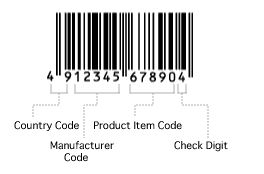
\includegraphics{Fig_Check_Bit}}  
	\centering
	\caption{Check-bit example}
	\label{fig:checkbit}
	\end{figure}


Calculation of Check Digit-
Last digit of a GTIN-13 barcode is the check-digit. To calculate check digit
$$ Check\ digit = 10 - mod \left[ 3\ *\ \left(Sum\ of\ odd\ digits + \ Sum\ of\ even\ digits \right),10 \right] $$

For the above example
\begin{equation}
\begin{split}
Check\ digit & = 10 - mod [ 3 * ((9+2+4+6+8+0) + (4+1+3+5+7+9)), 10] \\
               & = 10 - mod [174,10] \\
                & = 10 - 4 \\
                 & = 6               
\end{split}
\end{equation}
This can be seen as the last digit of the code.

\subsubsection*{Guassian Filter} \label{subsubsection:guassian_filter}

The Gaussian Smoothing Operator performs a weighted average of surrounding pixels based on the Gaussian distribution. It is used to remove Gaussian noise and is a realistic model of defocused lens. Gaussian filter is defined for both 1-dimensional space as well as 2-dimensional space. 

  \begin{figure}[h] 
	\centering
	\resizebox{14cm}{8cm}{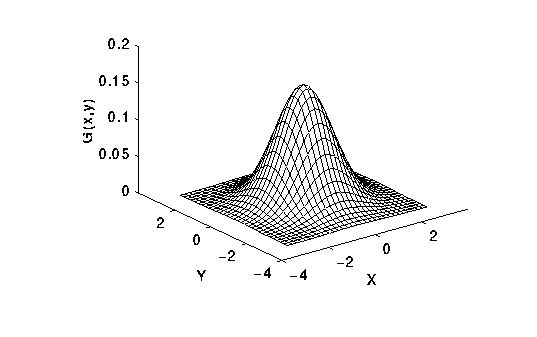
\includegraphics{Fig_Gaussian_Filter}}  
	\centering
	\caption{2-dimensional Guassian filter}
	\label{fig:guassian}
	\end{figure}

$$ g(x) = \frac{1}{\sigma \sqrt{2\pi}} * e^\frac{-x^2}{2\sigma^2} $$

where `$\sigma$' defines the amount of blurring

\section{Results and Discussion} \label{section:results}

The input video of moving object containing the barcode was applied to our algorithm on MATLAB. 
A 2 second input video was given. which produces 60 frames according to the camera specifications. The algorithm runs every function on each frame of the video until a barcode is read.

The following images shows the output obtained on MATLAB.


 \begin{figure}[!h] 
	\centering
	\resizebox{14cm}{8cm}{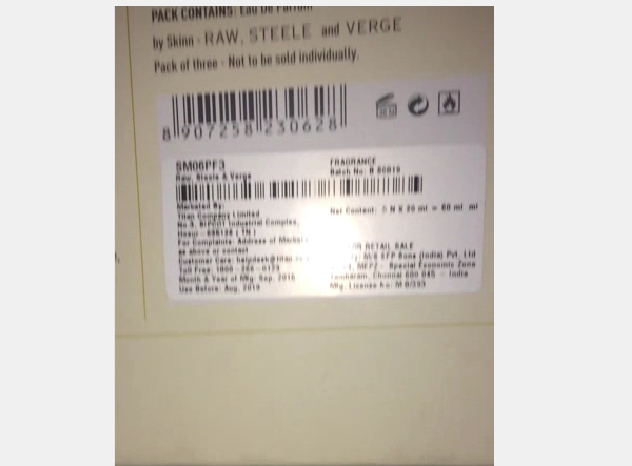
\includegraphics{Fig_Successful_Barcode}}  
	\centering
	\caption{Successful recognition of barcode}
	\label{fig:success_barcode}
	\end{figure}

The above image is the frame from which the barcode was successfully read. The value of k was found to be 9, which implies that 9th frame had a clear image of the barcode.

 \begin{figure}[!h] 
	\centering
	\resizebox{14cm}{8cm}{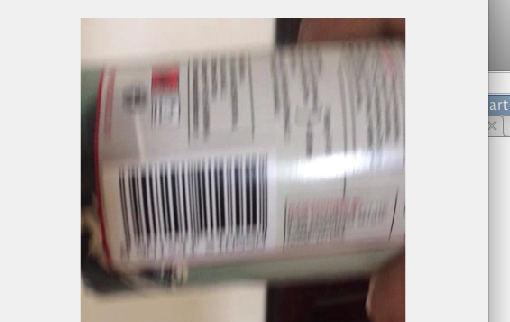
\includegraphics{Fig_Unsuccessful_Barcode}}  
	\centering
	\caption{Unsuccessful recognition of barcode}
	\label{fig:success_barcode}
	\end{figure}
	
	The above results suggest that a high-resolution camera is preferable to capture a video for a higher success rate of reading the barcode. It also suggests that the barcode is readable even with a considerable blur in the direction of motion when the barcode is perpendicular to that direction. On the other hand, any blur in the direction of the barcode is going to distort the bar width leading to faulty recognition or no recognition.

\section{Conclusion and Future Works} \label{section:conclusion}

 The ‘Smart Trolley’ looks like a feasible solution to eliminate long queues at super-markets. The prototype be improved in certain ways for a better shopping experience. Some of the ways where we can address a few drawbacks of the trolley are:

\begin{enumerate}
\item Use of multiple cameras: 4 cameras can reduce the work of the customer with the smart trolley. The disadvantage with using one camera is that the customer must manually look at the barcode and place it before the view of the camera. With 4 cameras, all four sides of a product are covered. This makes it simpler for the customer.
\item Use of other motion sensors other than ultra-sonic sensor: A method to form grid accurately only within the trolley and which is less susceptible to noise and external errors. The ultrasonic sensor is quite rigid and does not cover the entire trolley. There are several proximity sensors which can be chosen while making it into an embedded system.
\item Using OpenCV and python: OpenCV (Open Source Computer Vision) is a library of programming functions mainly aimed at real-time computer vision. This can be used as a tool better than the current one, MATLAB. OpenCV allows us to code in Python, which proves to be better than MATLAB in terms of speed and reliability. Also, using python allows us to use other micro-processors if they prove to be better.
\item Converting the prototype to a full functioning product: Once the prototype is tested for all possible test cases, it must be made into a finished product. For that, the software architecture should be resilient for several conditions like poor lighting, fast movement, horizontal scan, etc. The code must be converted in embedded C and a suitable processor which can handle the load must be decided upon. The whole product must be made into an ‘Attachable’ so that it can be fixed on any existing trolley.
\end{enumerate} 
 
 
 
 %%%%%%%%%%%%%%%%%%%%%%%%%%%%%%%%%%%%%%%%%%%%%%

%\begin{thebibliography}{10}
\bibliographystyle{unsrt}
\bibliography{Smart_Trolley}

%\end{thebibliography}

\end{document}



